% 2020 上海春季卷第 17 题；仅重绘原图可见线型与顶点标记，坐标为示意投影。
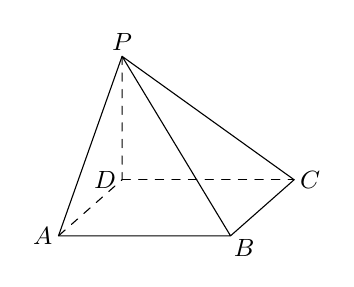
\begin{tikzpicture}[scale=.95,line cap=round,line join=round,font=\small]
  \coordinate (A) at (0,0);
  \coordinate (B) at (2.3,0);
  \coordinate (C) at (3.15,.75);
  \coordinate (D) at (.85,.75);
  \coordinate (P) at (.85,2.4);

  \draw[dashed] (P) -- (D) -- (A);
  \draw[dashed] (D) -- (C);
  \draw (P) -- (A) -- (B) -- (C) -- (P) -- (B);

  \node[above,inner sep=2pt] at (P) {$P$};
  \node[left,inner sep=2pt] at (A) {$A$};
  \node[below right,inner sep=1pt] at (B) {$B$};
  \node[right,inner sep=2pt] at (C) {$C$};
  \node[left,inner sep=2pt] at (D) {$D$};
\end{tikzpicture}
